The primary result of this project is a synthetic image dataset generated using Unity, offering an alternative to real-world images for training and testing machine learning models. The dataset consists of 2350 images with various boats and maritime objects in a harbor environment. It showcases the capabilities of the Unity Perception package, including the use of diverse scenarios with varying camera positions, weather effects and object orientations. These features increase the dataset's diversity for machine learning tasks, helping to create better models. A link to the GitHub repository containing the dataset and additional resources can be found in Appendix A.

\section{Dataset}
The dataset contains synthetic images of objects in a harbor environment, created entirely using Unity. Objects in the dataset include boats, sailboats, kayaks and buoys, with variations in environmental conditions such as rain.\\

\noindent The distribution of object types and their corresponding weather conditions is summarized in Table~\ref{tab:dataset_composition}. Each object type has been rendered under various conditions to ensure a realistic and comprehensive dataset for training machine learning algorithms.
 
\begin{table}[H]
\centering
\begin{tabular}{|l|c|}
\hline
\multicolumn{2}{|c|}{\textbf{Dataset Distribution}} \\ 
\hline
\textbf{Object Type} & \textbf{Total Appearances}\\ 
\hline
Boats         & 2100  \\ 
Small rib     & 200 \\
Sailboat      & 900     \\
Sailboat without sail     & 800    \\
Kayak        & 1100     \\ 
Buoy         & 200     \\ 

\hline
\textbf{Total}       & \textbf{5300} \\ 
\hline
\end{tabular}
\caption{Breakdown of the dataset by object type.}
\label{tab:dataset_composition}
\end{table}



\begin{figure}[H]
\centering
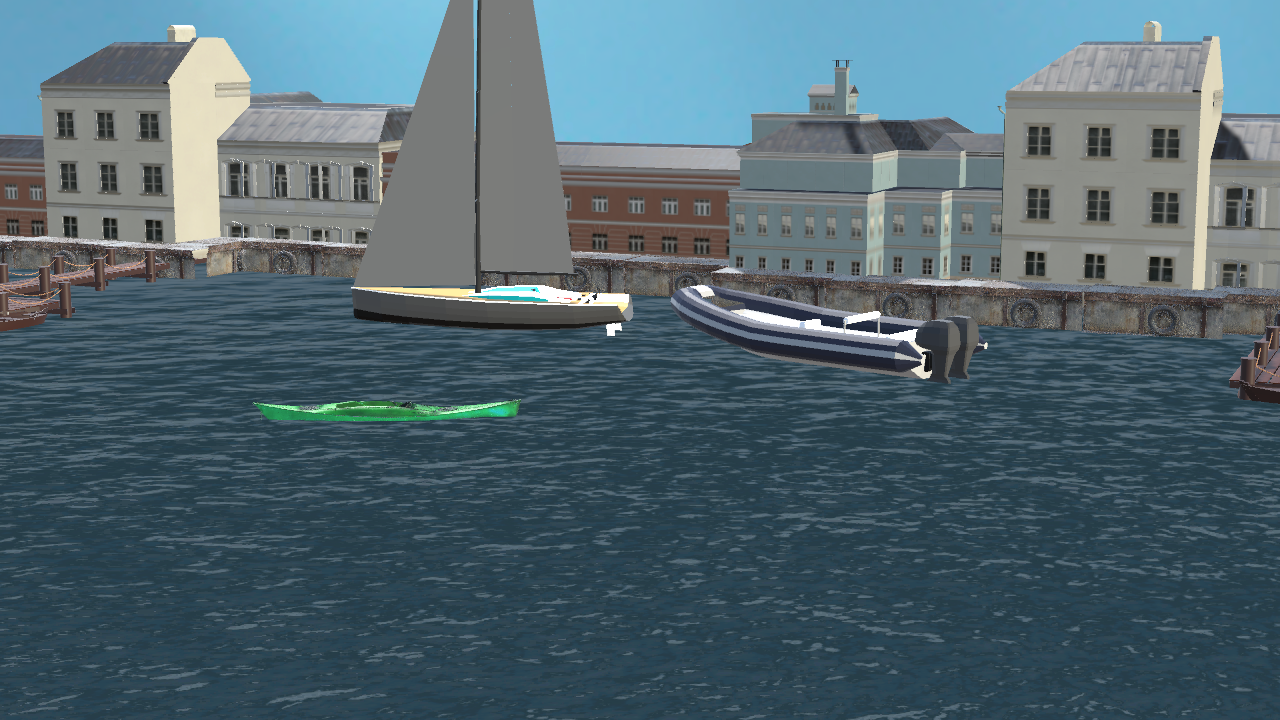
\includegraphics[width=0.8\textwidth]{Figures/results/rand2.png}
\caption{Example of one of the images in the dataset.}
\label{fig:original_image}
\end{figure}

\section{Dataset Diversity}
A key goal of this project was to create a dataset that captures a wide range of scenarios. The results demonstrate a highly varied dataset with changes in object rotations, positions and weather conditions. Ensuring diversity in the dataset helps make it more generalizable, improving model performance in different situations. However, one aspect that could be further improved is the variety of backgrounds, which is quite similar in all the images. \\

\noindent Figure \ref{fig:randomized_images} shows examples of randomized images with the same target object. These examples highlight how randomization creates variety in rotation, background and camera position.

\begin{figure}[H]
\centering
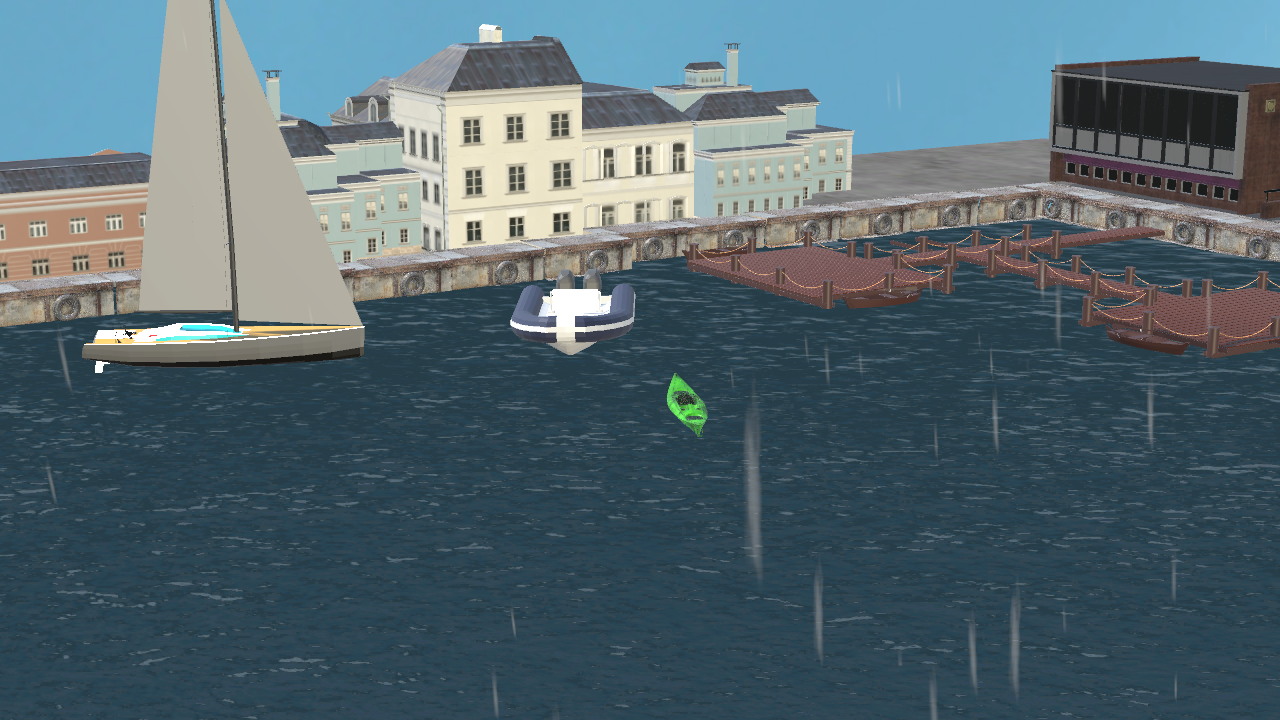
\includegraphics[width=0.32\textwidth]{Figures/results/rand1.png}
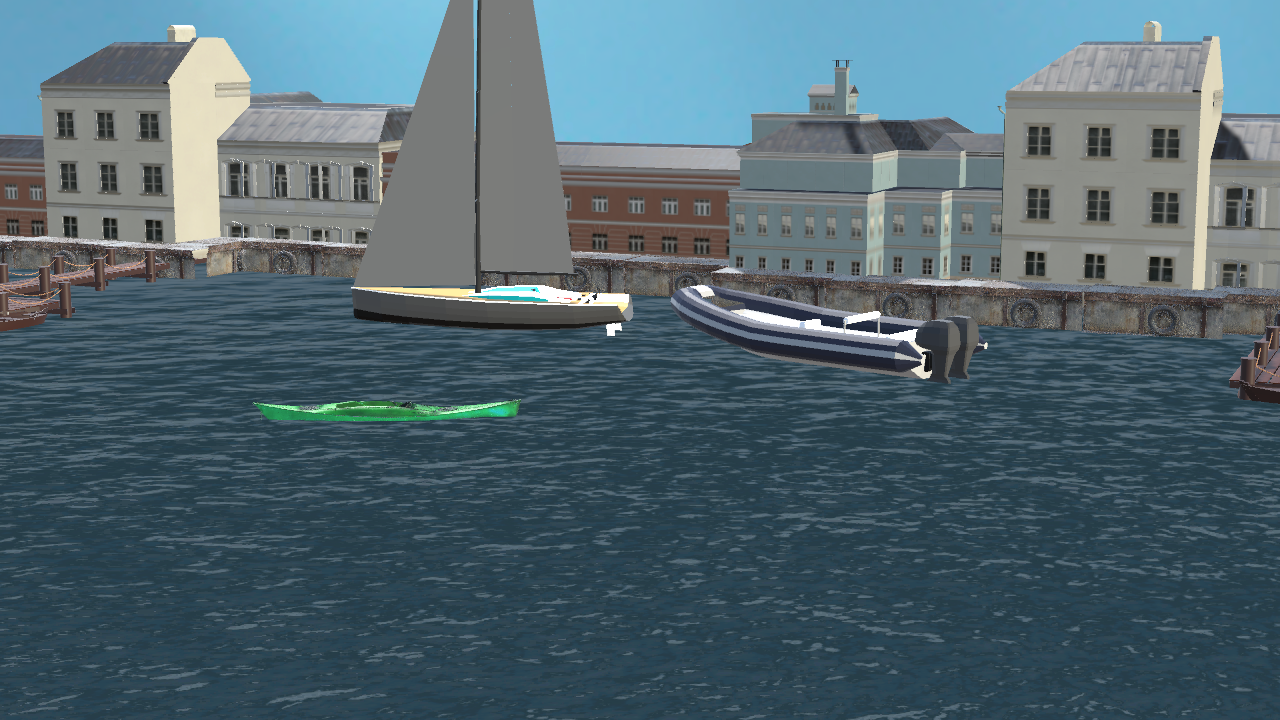
\includegraphics[width=0.32\textwidth]{Figures/results/rand2.png}
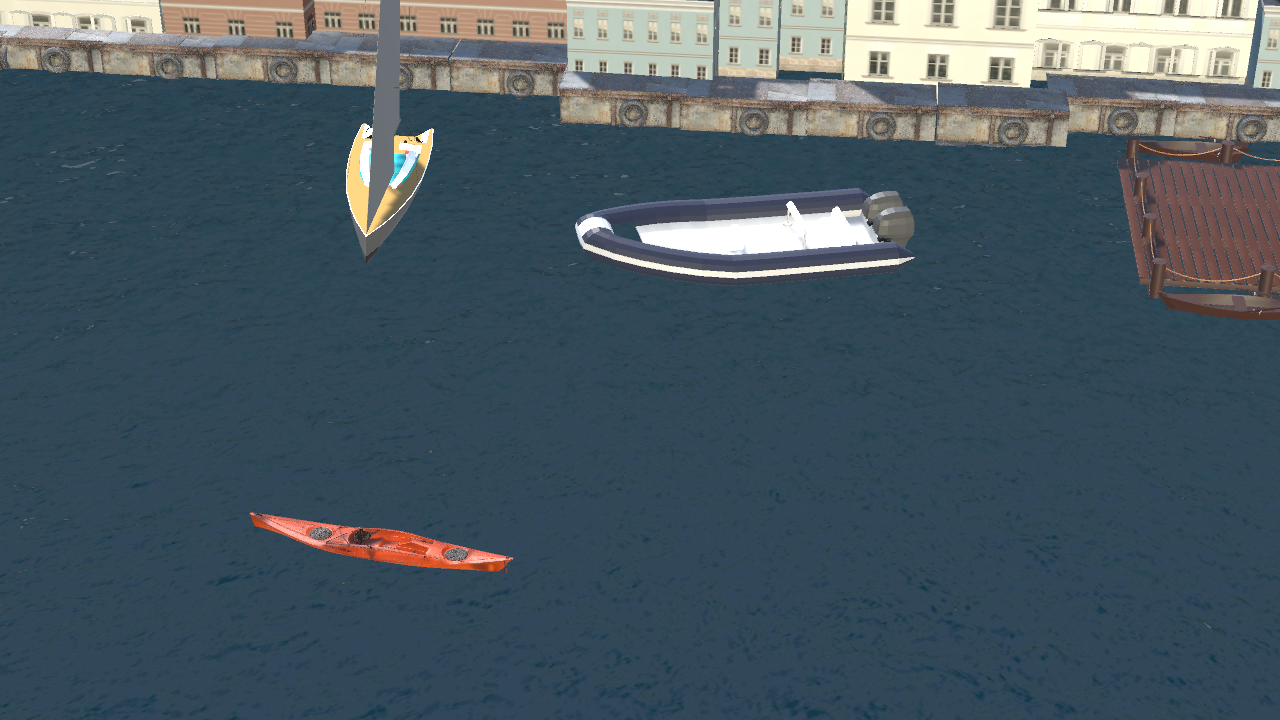
\includegraphics[width=0.32\textwidth]{Figures/results/rand3.png}
\caption{Example of 3 randomized images with the same target.}
\label{fig:randomized_images}
\end{figure}

\section{Labeling}
Labeling is important because it helps computer vision models identify and learn the objects in an image \cite{Labelling}.  The results from the generation included two images for each scene: the original image and a corresponding segmentation image, where each object is marked with a distinct color. This dual-image output provides a clear connection between the visual data and the labels, ensuring consistency in training.\\

\noindent Figure \ref{fig:labeled_images} shows an example of the labeling process. The left image is the original and the right image is the segmented version. This comparison shows how well the labels match the objects in the original image, ensuring the model learns from accurate data.

\begin{figure}[H]
\centering
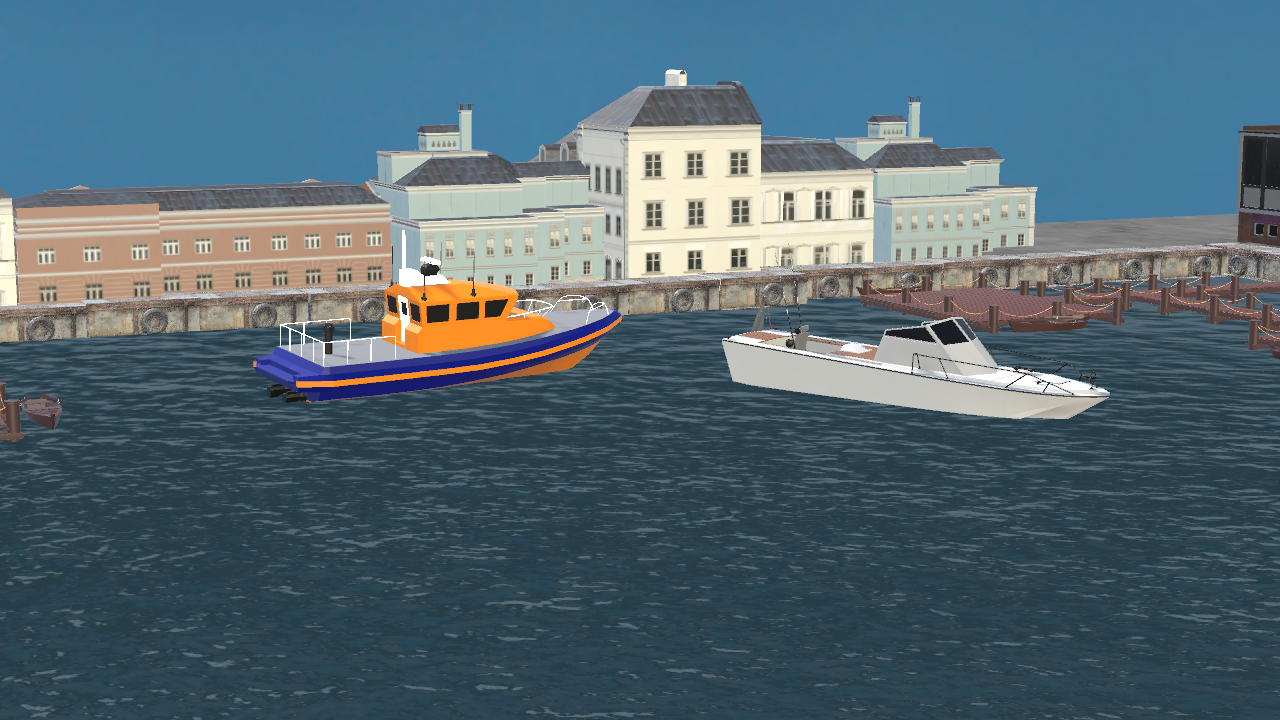
\includegraphics[width=0.49\textwidth]{Figures/results/rgb_105.png}
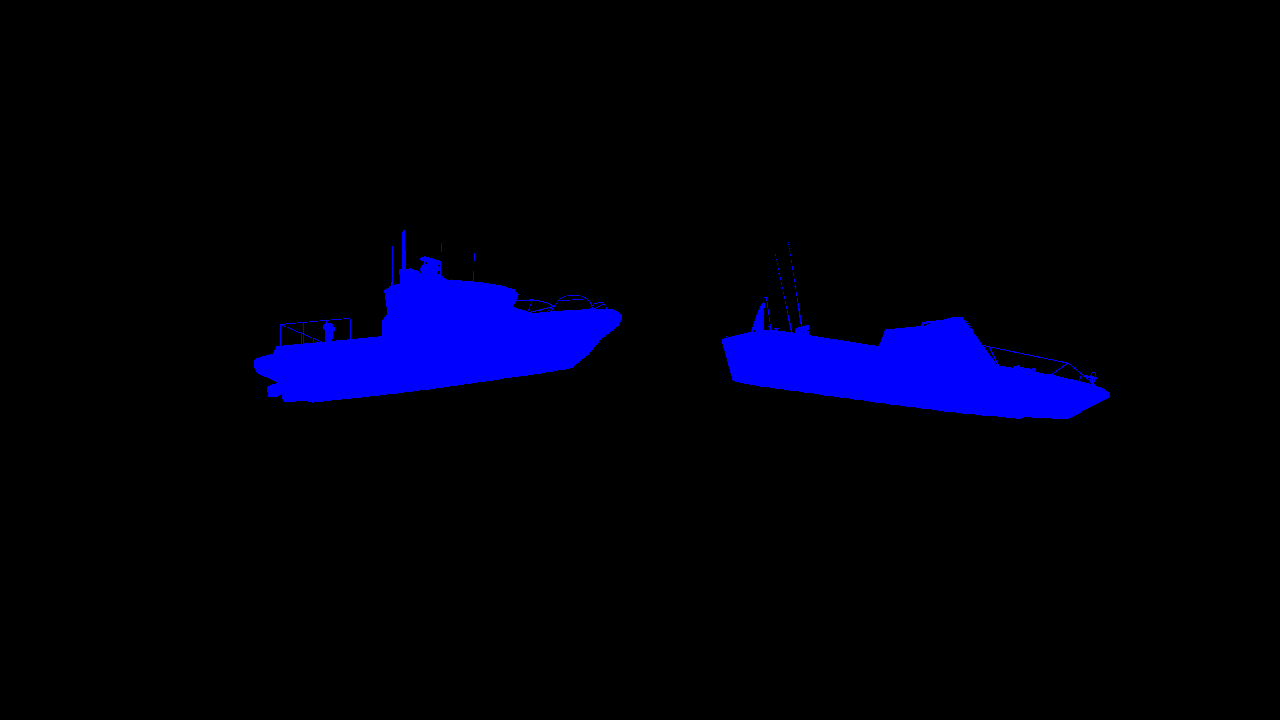
\includegraphics[width=0.49\textwidth]{Figures/results/segmentation_105.png}
\caption{Comparison of the original image and its labeled segmentation output.}
\label{fig:labeled_images}
\end{figure}

